\chapter{Linkbudget}\label{ch:linkbudget}

\section{ADS-B signals}
Automatic dependent surveillance-broadcast (ADS-B) is a system in which aircraft continually transmit their identity and GPS-derived navigational information. ADS-B networks for air traffic monitoring have already been implemented in areas around the world, but ground stations cannot be installed in mid-ocean and are difficult to maintain in the Arctic, leaving a coverage gap for oceanic and high latitude airspace \citep{FlyingLab}. Therefore a solution can be to monitor the signals with a low orbit satellite using an antenna matched to the frequencies of the ADS-B.There are currently three types of ADS-B transmissions, including the 1090 MHz extended squitter (ES), the 978 MHz universal access transceiver (UAT), and the VHF data link (VDL) mode 4 operating between 108 and 137 MHz.
 \\
An ADS-B message is 112 bits long and the transmission takes 120us. The mudulation is pulsed RF and the package consist of 5 parts. The first part is Downlink Format which tells that this is an ADS-B signal, second part is Additional Identifier which has different meaning within each ADS-B subtype. The third is the ICAO which is the unique identifier of the aircraft. The fourth is the DATA which contains several informations including aircraft operation status, airborne position and velocities measured from different sensors. The fifth and last is the checksum \citep{Modesorg}. It is observed that the ADS-B signal is a unencrypted signal which makes it easy to detect and therefore also vulnerable to attacks \citep{Attacks}.       

\begin{figure}[h]
\centering 
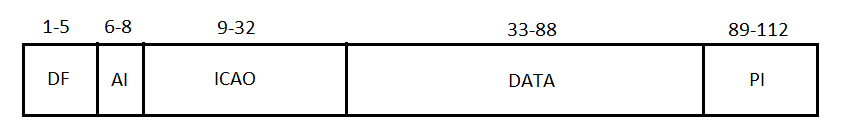
\includegraphics[scale = 0.5]{figures/adsb_signals/adsb_message.png}
\caption{112 bit long ADS-B message}
\label{fig:adsb_mes}
\end{figure}


\textbf{1090MHz Mode S Extended Squitter}\\
This is the most common frequency in ADS-B. It uses a single channel at 1090MHz and is used for communication from aircraft to ground only. The message is sent in intervals determined by the aircraft commonly every second.   
\\
\textbf{978MHz Universal Acces Transceiver}\\
This is a newer standard that communicates from aircraft to aircraft. It uses a single frequency at 978MHz.  
\\
\textbf{108-137MHz VHF Data Link Mode 4}\\
This is most commonly used at small airplanes. It is multi-channel where the frequency depends upon the local regulations. The channel spacing is 1MHz. 

\section{Free space loss}

Typically in satellite communication a LOS component exist. Therefore the only obstacle between the satellite and user is the atmosphere and therefore the loss can be modelled as free space, with a limited variation due to weather conditions. ADS-B signal is sent through a linear polarized monopol with power varying from 75 W to 500 W depending of the airplane and speed \citep{FlyingLab}. The height of a Low Earth Orbit (LEO) satellite is between 600 km to 800 km. To calculate the power loss Friis Transmission Equation is used. 

\begin{equation}
\frac{P_r}{P_t} = (\frac{\lambda}{4\pi R})^2 G_t G_r|\vec{Pr}\cdot \vec{Pt}|^2
\end{equation}

\begin{equation}
\lambda = \frac{c}{f}
\end{equation}
Where $c = 3e8$ is speed of light in vaccum and $ f$ is the frequency in Hz. $|\vec{Pr}\cdot \vec{Pt}|^2$ denotes polarization mishmash. When solving for $f = 137MHz$ $R=800km$  $G_t = 0 dB$ and a polarization loss at 0, the free-space loss becomes 133.2dB.

\section{LEO coverage}
For a satellite the coverage area on the earth is a circular area which is defined by the height (H) of the satellite and the angel $\alpha_0$ which is half the -3dB beam width of the antenna for the satellite. The maximum distance the signal travels from the satellite to the earth and vice versa, is d which is depicted in figure \ref{fig:cov_sat} \citep{Cakaj2014}. The equation for d is given by equation \ref{eq:dist} 

\begin{equation}
d=R_e(\sqrt{(\frac{H+R_e}{R_e})^2-\cos^2{\epsilon_0}}-\sin{\epsilon_0})
\end{equation}
\label{eq:dist}

Where

\begin{equation}
\epsilon_0 = \arccos{\frac{\sin{\alpha_0}(R_e+H)}{R_e}}
\end{equation}
\label{eq:dist2}

and $R_e = 6378km$ is the radius of the earth. Further the coverage percentage of the satellite can be calculated by equation \ref{eq:coverage} which uses the total area of the earth divided by the area covered by the satellite. 

\begin{equation}
Coverage(\%) = \frac{A_{coverage}}{A_{earth}} = \frac{2 \pi R_e^2 ( 1 - \cos{\beta_0})}{4 \pi R_e^2}\cdot 100\%
\end{equation}
\label{eq:coverage} 

\begin{equation}
\beta_0 = 90 - \alpha_0 -\epsilon_0
\end{equation}

For a LEO with a height of $H = 800km$ and $\alpha_0 = 15^\circ$ the distance becomes $d = 859km$ and with a coverage percentage of $Coverage = 0.053 \%$

\begin{figure}[H]
\centering 
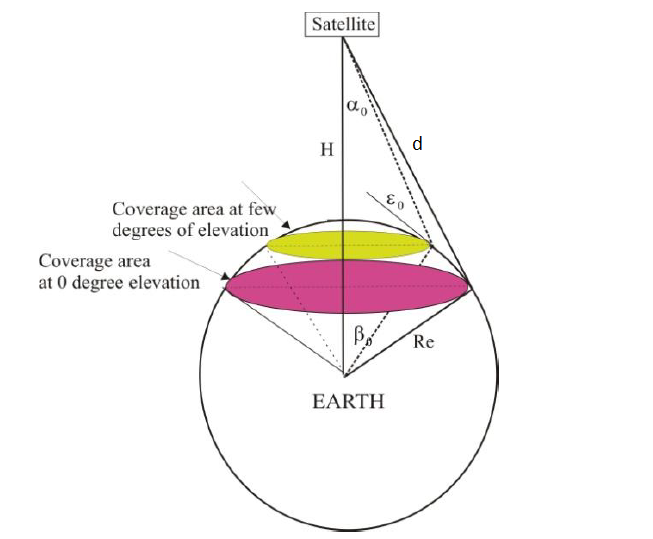
\includegraphics[scale = 0.7]{figures/linkbudget/sat_coverage.png}
\caption{Earth coverage for a satellite. Pink area is maximun coverage, green is area limited to the antenna beamwidth. \citep{Cakaj2014}}
\label{fig:cov_sat}
\end{figure} 

Because of the geometry of the earth and the height of the satellite a maximum coverage area must exist. This is depicted in figure \ref{fig:cov_sat} as purple area. To find the maximum angle $\alpha_0$ equation \ref{eq:max_cov} is used. At a height at $H=800km$ the maximum angle becomes $62.7^\circ$ which gives a maximum distance $d = 3040km$ and a coverage percentage at $Coverage = 4.7\%$.

\begin{equation}
\alpha_0(max) = \arcsin{\frac{R_e}{R_e+H}}
\end{equation}
\label{eq:max_cov} 

\section{LEO radiation pattern}
Because of the unknown factor of which direction the signal arrives and which polarization the signal has, a circular polarized antenna is best suited for satellite communication \citep{Balanis2005}. Depending on the application it can ether be the ground station or satellite which polarization is circular. In this project it is desired to have the circular antenna placed at the satellite because ADS-B signals is transmitted by a linear dipole \citep{itu2017}. As described earlier the signal does not always travel the same distance and therefore the loss is diffrent due to the angle of reception. The farfield of the satellite antenna should therefore compensate for this by letting the gain increase due to the angle which is depicted in figure \ref{fig:sat_farfield}.   

\begin{figure}[H]
\centering 
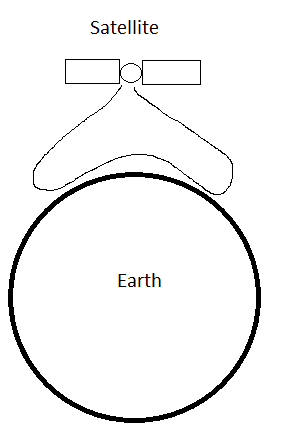
\includegraphics[scale = 0.7]{figures/linkbudget/sat_farfield.png}
\caption{Desired farfield for a LEO satellite}
\label{fig:sat_farfield}
\end{figure} 

Knowing equation \ref{eq:dist} and \ref{eq:dist2} a polar plot of the farfield can be calculated. This is done by equation \ref{eq:coverage_farfield} where $d(\alpha_0)$ is equation \ref{eq:dist}. The formula normalizes the gain to an angle of zero. A 2D polar plot 
is depicted in figure \ref{fig:sat_farfield_polar} for $f=122.5MHz$, $H=800km$ and $\alpha_{max} = 62.7^{\circ}$. It is seen that in the $\alpha_{max}$ direction a gain of 12dB is required. It is also seen from the equation that the loss due to the angle is frequency independent.  
  
\begin{equation}
Gain_{required} = -10\cdot log_{10}(\frac{(\frac{\lambda}{4 \pi d(\alpha) })^2}{(\frac{\lambda}{4 \pi d(0) })^2}) = -10\cdot log_{10}(\frac{d(0)^2}{d(\alpha)^2})
\end{equation}
\label{eq:coverage_farfield} 

\begin{figure}[H]
\centering 
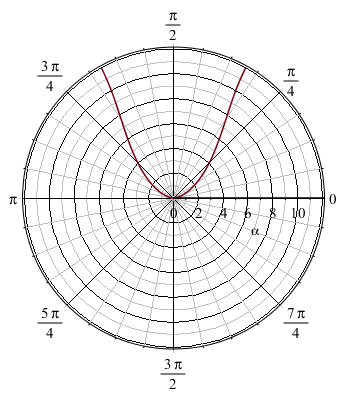
\includegraphics[scale = 1]{figures/linkbudget/sat_farfield_polar.png}
\caption{Desired farfield for a LEO satellite}
\label{fig:sat_farfield_polar}
\end{figure} 

\section{Tabels}
With the previously description is it now easy to calculate a linkbudget. It is assumed that the receiving antenna is a circular polarized antenna which will cause a polarization mismatch at -3dB \citep{Balanis2005}. Futher an atmospheric loss at 0.1dB is assumed together with a carier to noise radio at minimum 9dB \citep{itu2017}. The system noise temperature is set to 373K because of the high temperature span in the LEO \citep{FlyingLab}. The calculations is done at a transmit power at 75W which is the minimum due to the standard. Normally when planes are over the sea the transmit power is increased up to 500W.   
 
\begin{center}
\captionof{table}{Linkbudget for 1090MHZ and H = 800km} \label{tab:1090}
  \begin{tabular}{ l  l  l  l  l}
    \hline
   \textit{Item} & \textit{Link parameter} & \textit{Value} & \textit{Unit} & \textit{Computation} \\ \hline
    1 & Frequency	& 1090 & MHz & \\ \hline
    2 & Transmit power (75W) & 18.8 & dB & \\ \hline
    3 & Transmit antenna gain & 3 & dBi & \\ \hline
    4 & Athmospheric absorbtion (clean air) & 0.1 & dB & \\ \hline
    5 & Free-space loss & 151.2 & dB & \\ \hline
    6 & Polarisation loss & 3 & dB & \\ \hline
    7 & Received carrier power & -129.6 & dB & 2+3-4-5\\ \hline
    8 & Bandwith (4.6MHz) & 66.6 & dB Hz & \\ \hline 
    9 & System noise temperature (373K) & 25.7 & dBK& \\ \hline 
    10 & Boltzmann's constant & -228.6 & dBW/Hz/K& \\ \hline 
    11 & Noise power & -136.6 & dBW& 8+9+10\\ \hline 
    12 & Carrier to noise ratio & 7.0 & db & 7-11\\ \hline 
    13 & C/(N+I) & 9 & db & Requirement\\ \hline
    14 & Minimum receive antenna gain at $\alpha_0 = 0 $ & 2.0 & db & 13-12\\ \hline
    15 & Minimum receive antenna gain at $\alpha_0 = \alpha_{max} $ & 14.0 & db & 14+equation \ref{eq:max_cov} \\ \hline  \end{tabular}
\end{center}


\begin{center}
\captionof{table}{Linkbudget for 978MHZ and H = 800km} \label{tab:978}
  \begin{tabular}{ l  l  l  l  l}
    \hline
   \textit{Item} & \textit{Link parameter} & \textit{Value} & \textit{Unit} & \textit{Computation} \\ \hline
    1 & Frequency	& 978 & MHz & \\ \hline
    2 & Transmit power (75W) & 18.8 & dB & \\ \hline
    3 & Transmit antenna gain & 3 & dBi & \\ \hline
    4 & Athmospheric absorbtion (clean air) & 0.1 & dB & \\ \hline
    5 & Free-space loss & 150.3 & dB & \\ \hline
    6 & Polarisation loss & 3 & dB & \\ \hline
    7 & Received carrier power & -128.6 & dB & 2+3-4-5\\ \hline
    8 & Bandwith (4.6MHz) & 66.6 & dB Hz & \\ \hline 
    9 & System noise temperature (373K) & 25.7 & dBK& \\ \hline 
    10 & Boltzmann's constant & -228.6 & dBW/Hz/K& \\ \hline 
    11 & Noise power & -136.6 & dBW& 8+9+10\\ \hline 
    12 & Carrier to noise ratio & 8.0 & db & 7-11\\ \hline 
    13 & C/(N+I) & 9 & db & Requirement\\ \hline
    14 & Minimum receive antenna gain at $\alpha_0 = 0 $ & 1.0 & db & 13-12\\ \hline
    15 & Minimum receive antenna gain at $\alpha_0 = \alpha_{max} $ & 13.0 & db & 14+equation \ref{eq:max_cov} \\ \hline
  \end{tabular}
\end{center}

\begin{center}
\captionof{table}{Linkbudget for 122.5MHZ and H = 800km} \label{tab:122.5}
  \begin{tabular}{ l  l  l  l  l}
    \hline
   \textit{Item} & \textit{Link parameter} & \textit{Value} & \textit{Unit} & \textit{Computation} \\ \hline
    1 & Frequency	& 122.5 & MHz & \\ \hline
    2 & Transmit power (75W) & 18.8 & dB & \\ \hline
    3 & Transmit antenna gain & 3 & dBi & \\ \hline
    4 & Athmospheric absorbtion (clean air) & 0.1 & dB & \\ \hline
    5 & Free-space loss & 132.3 & dB & \\ \hline
    6 & Polarisation loss & 3 & dB & \\ \hline
    7 & Received carrier power & -110.6 & dB & 2+3-4-5\\ \hline
    8 & Bandwith (1MHz) & 60.0 & dB Hz & \\ \hline 
    9 & System noise temperature (373K) & 25.7 & dBK& \\ \hline 
    10 & Boltzmann's constant & -228.6 & dBW/Hz/K& \\ \hline 
    11 & Noise power & -142.9 & dBW& 8+9+10\\ \hline 
    12 & Carrier to noise ratio & 32.3 & db & 7-11\\ \hline 
    13 & C/(N+I) & 9 & db & Requirement\\ \hline
    14 & Minimum receive antenna gain at $\alpha_0 = 0 $ & -23.3 & db & 13-12\\ \hline
    15 & Minimum receive antenna gain at $\alpha_0 = \alpha_{max} $ & -11.3 & db & 14+equation \ref{eq:max_cov} \\ \hline
  \end{tabular}
\end{center}
